\makeheading{Week 1}{\daterange{2021-09-08}{2021-09-10}}%chktex 8
\setcounter{section}{-1}
\section{Module 0: Introduction to Biostatistics}
\begin{Regular}{Course Goal}
    Understand common epidemiological study designs and basic biostatistical analysis
    methods that can be used to answer questions in health research.
\end{Regular}
\subsection*{Every day we make decisions that affect our health and wellness\footnote{Headlines taken from \href{http://www.cbc.ca/news/health}{CBC} on \printdate{2018-04-30}.}}%chktex 8
\begin{itemize}
    \item \textbf{Exercise lowers risk of depression at all ages, researchers find.}
          \begin{itemize}
              \item 150 minutes of activity each week is beneficial, but doing less still has positive effects.\\
                    \emph{Amina Zafar · CBC News · Posted:  \printdate{2018-04-24} | Last Updated: \printdate{2018-04-24}.}%chktex 8
          \end{itemize}
    \item \textbf{Fewer hospital stays for asthma reported for Canadian children and teens.}
          \begin{itemize}
              \item Research says more than half with asthma don't have it under control.\\
                    \emph{CBC News · Posted: \printdate{2018-04-26} | Last Updated: \printdate{2018-04-26}.}%chktex 8
          \end{itemize}
    \item \textbf{Prescription to slow worsening myopia in Canadian kids? Head outdoors.}
          \begin{itemize}
              \item Nearly \qty{130}{\percent} of children 11 to 13 are near-sighted, study finds.\\
                    \emph{CBC News · Posted: \printdate{2018-04-21} | Last Updated: \printdate{2018-04-23}.}%chktex 8
          \end{itemize}
    \item \textbf{Opioid-related deaths nearly tripled in Ontario from 2000-2015.}%chktex 8
          \begin{itemize}
              \item It's time `to get past the stigma of drug use being among addicts,' scientist says.\\
                    \emph{The Canadian Press · Posted: \printdate{2018-04-27} | Last Updated: \printdate{2018-04-27}.}%chktex 8
          \end{itemize}
    \item \textbf{EU member states urged to develop co-ordinated vaccine plans for measles, flu, and other diseases.}
          \begin{itemize}
              \item Several EU nations are facing unprecedented outbreaks of measles --- a highly contagious disease that can kill.\\
                    \emph{Thomson Reuters · Posted: \printdate{2018-04-26} | Last Updated: \printdate{2018-04-26}.}%chktex 8
          \end{itemize}
    \item \textbf{Lung cancer patients live longer with immune therapy, study suggests.}
          \begin{itemize}
              \item Immune therapy treatments worked for only about half of patients, but that's far better than chemo has done.\\
                    \emph{The Associated Press · Posted: \printdate{2018-04-16} | Last Updated: \printdate{2018-04-16}.}%chktex 8
          \end{itemize}
\end{itemize}
\subsection*{Formulating a Research Question\footnote{News Article: \href{https://www.cbc.ca/news/health/keytruda-1.4621895}{https://www.cbc.ca/news/health/keytruda-1.4621895}}\footnote{Original paper: \href{https://www.nejm.org/doi/full/10.1056/NEJMoa1801005}{https://www.nejm.org/doi/full/10.1056/NEJMoa1801005}}}
\begin{paragraph}{Lung cancer patients live longer with immune therapy, study suggests.}
    Immune therapy treatments worked for only about half of patients, but that's far better than chemo has done.\\
    \emph{The Associated Press · Posted: \printdate{2018-04-16} | Last Updated: \printdate{2018-04-16}.}%chktex 8
\end{paragraph}
\begin{itemize}
    \item \textbf{Population}: Patients diagnosed with lung cancer (advanced non-small-cell lung cancer with no previous treatment).
    \item \textbf{Exposure}: Treatment with Immune therapy (with chemo vs chemo alone).
    \item \textbf{Outcome}: Overall survival.
    \item \textbf{Timeframe}: One year following diagnosis (study was conducted \printdayoff\daterange{2016-02-00}{2017-03-00}).%chktex 8
\end{itemize}
\subsection*{Example: Electronic cigarette use and smoking}
\begin{Example}{}
    \textbf{Research Question}: Is e-cigarette usage in youth associated with the initiation of
    cigarette smoking?
\end{Example}
\begin{itemize}
    \item Consider the following paper recently published by UW researchers.
    \item The full text of the paper is available through the course e-reserves.
\end{itemize}
\begin{figure}[H]
    \centering
    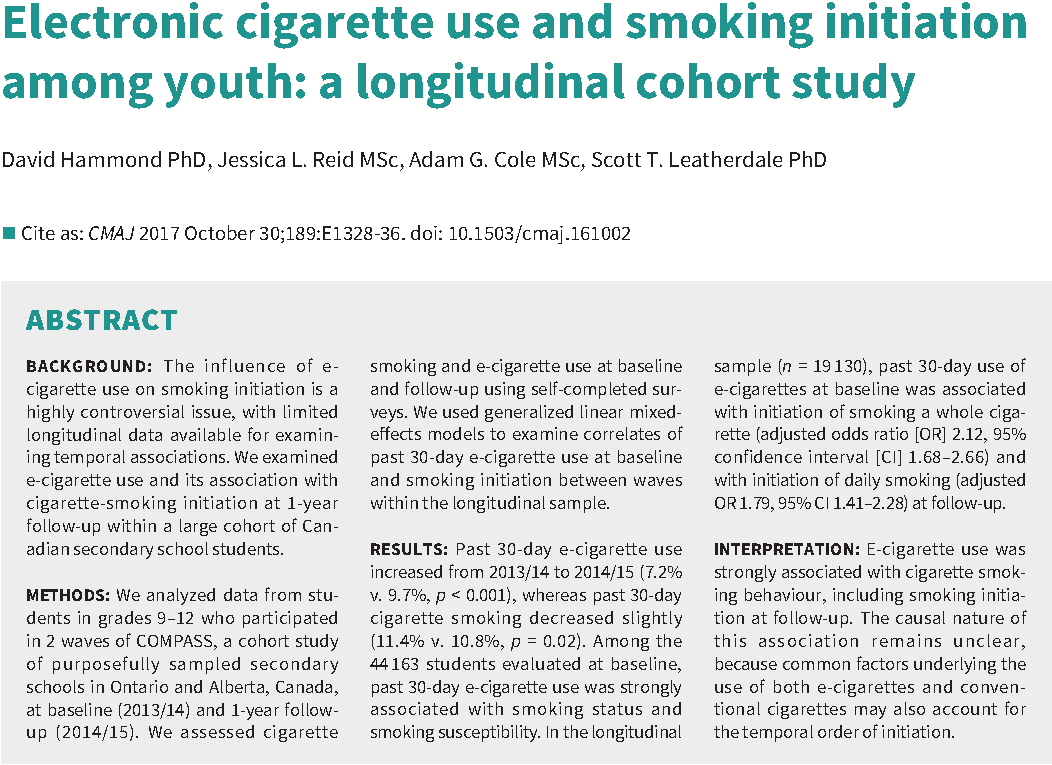
\includegraphics[width=0.9\textwidth]{0/1.pdf}
\end{figure}
\begin{itemize}
    \item \textbf{Population}: Canadian secondary school students (age 15--19, grade 9--12 in Alberta and Ontario).
    \item \textbf{Exposure}: E-cigarette usage at baseline (2013/14 school year).
    \item \textbf{Outcome}: Cigarette smoking initiation 1-year later (by 2014/15 school year).
    \item \textbf{Timeframe}: One year of follow-up.
\end{itemize}
\begin{figure}[H]
    \centering
    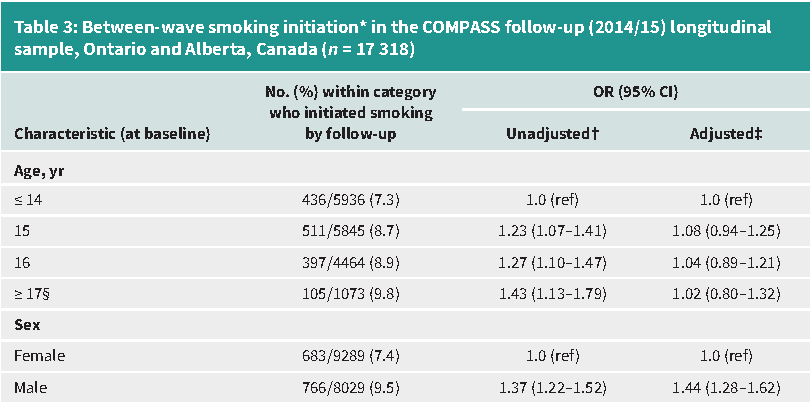
\includegraphics[width=0.9\textwidth]{0/2.pdf}
    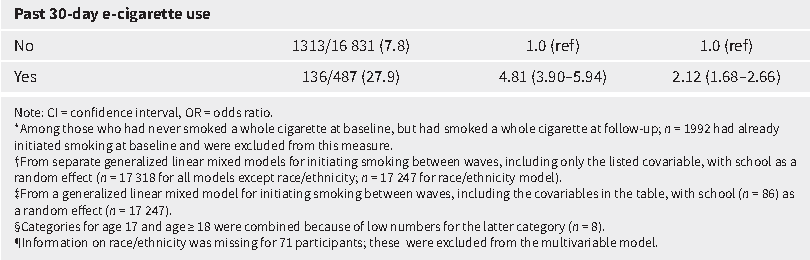
\includegraphics[width=0.9\textwidth]{0/3.pdf}
\end{figure}
\subsection*{Example Data Analysis (Module 2)}
\begin{table}[H]
    \centering
    \begin{NiceTabular}{cc|c|c|c}
        \Block{1-5}{Smoking Initiation Status}\\%chktex 8
        \Block{1-5}{\quad\qquad$D+$\quad\; $D-$} \\%chktex 8
        \cmidrule{3-4}
        \multirow{2}{*}{E-cig Usage} & $ E+ $ &  136 & 351 & 487$\to$\qty{27.9}{\percent}        \\
        \cmidrule{3-4}
        & $ E- $ &  1313 & 15518 & 1638$\to$\qty{7.8}{\percent}                                       \\
        \cmidrule{3-4}
    \end{NiceTabular}
\end{table}
\[ \text{Relative Risk}=\frac{136/487}{1313/16831}=3.58 \]
Youth who used e-cigarettes had 3.58 times the rate of smoking initiation one year
later versus those who did not use e-cigarettes.
